\section{Different optimization strategies}
\subsection{Change components of the initial architecture}

\begin{frame}{Batch Normalization, Dropout layers, activation function and pooling}
	\begin{itemize}
		\item Batch normalization to speed up the training \cite{BatchNorm2015}
		\item Initial activation function: $\mathrm{ReLu}: \mathbb{R} \to \mathbb{R}_0^+, x \mapsto \max\{0,x\}$, still MSE of over 15 on the testing 
		set, less then 2 on the training set\\
		$\Rightarrow$ Overfitting problems
		\item Dropout layers \cite{Dropout2014} to make the model more robust and reduce overfitting
		%build in one with dropout probability $p=0.5$
		\item Solve problems of dead neurons using
		\begin{align*}
		\mathrm{leakyReLU} : \mathbb{R} \to \mathbb{R}, x \mapsto \begin{cases}
		x, x \geq 0\\
		c \cdot x, x <0
		\end{cases}
		\end{align*}
		with $c = 0.01$, MSE of around 11 on the testing set and less than 3 on the training set
	\end{itemize}
\end{frame}

\begin{frame}{Pooling layers (initial splitting)}
	\begin{table}[!t]
		\normalsize
		\centering
		\begin{tabular}{lcccc}
			\toprule
			\multirow{2}{*}{Initial splitting, 8 epochs}  & \multicolumn{2}{c}{$\mathrm{ReLU}$} & \multicolumn{2}{c}{$\mathrm{leakyReLU}$} \\
			& Train & Test & Train & Test\\
			\midrule
			No pooling & 2.85 & 12.08 & 2.45 & 10.75 \\
			Max pooling & 5.62 & 11.82 & 5.52 & 10.29 \\
			Max pooling (15 epochs) & - & - & \textbf{3.22} & \textbf{9.63} \\
			Average pooling & 7.70 & 11.40 & 6.08 & 13.09\\
			\bottomrule
		\end{tabular}
		\caption{MSE results of the network using different pooling strategies, one dropout layer, two different activation functions and 
			the initial splitting. We trained each of the models for eight epochs.}
	\end{table}
\end{frame}

\subsection{Siamese approach}

\begin{frame}{Siamese Architecture: Setup}
	\begin{itemize}
		\item Based on the initial architecture
		\item Using the same convolutional layers on raw frame and optical flow
		\item Weighted sum of the results into fully connected layers
	\end{itemize}
	\begin{center}
	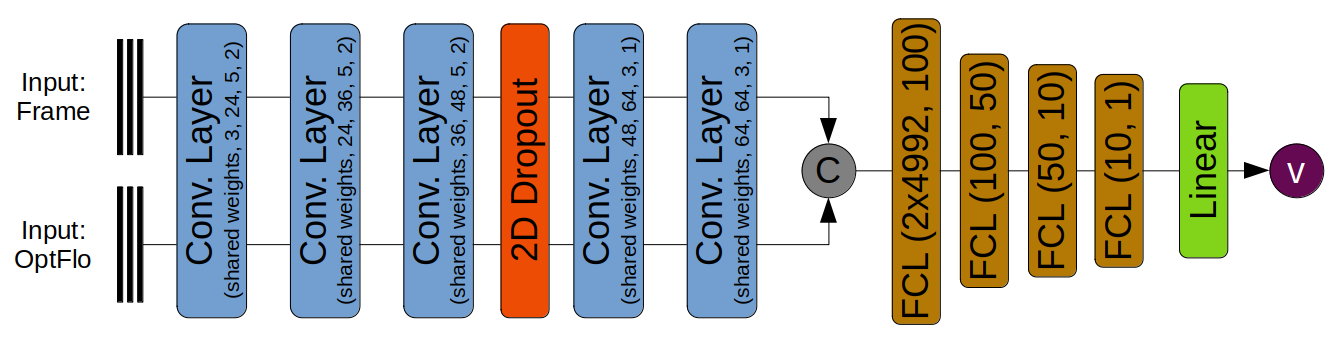
\includegraphics[width=0.8\textwidth]{imgs/siamese_model.png}
	\end{center}
	\begin{itemize}
		\item Use model also for two consecutive frames $f_t$ and $f_{t+1}$\\
		$\Rightarrow$ advantage: no previous calculation of optical flow needed
	\end{itemize}
\end{frame}

\begin{frame}{Siamese Architecture: Performance}
	\textbf{Performance (Siamese network frame with optical flow):}
	\begin{columns}[c]
		\begin{column}{0.5\textwidth}
			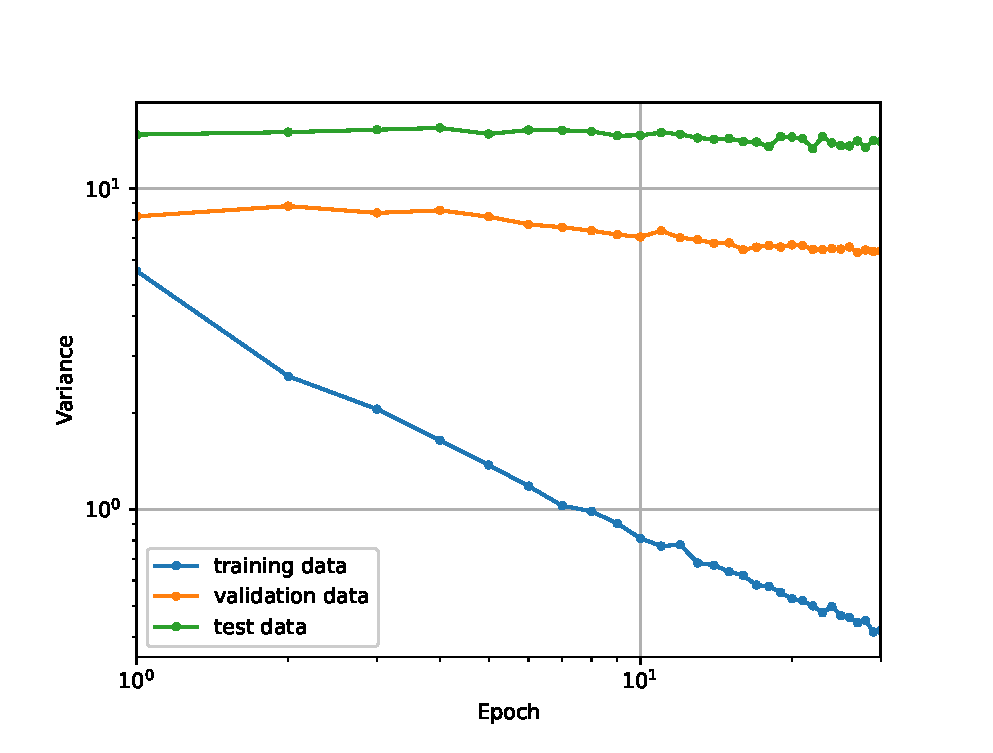
\includegraphics[width=\textwidth]{imgs/siamese_fof_trainingprocess.eps}
		\end{column}
		\begin{column}{0.5\textwidth}
			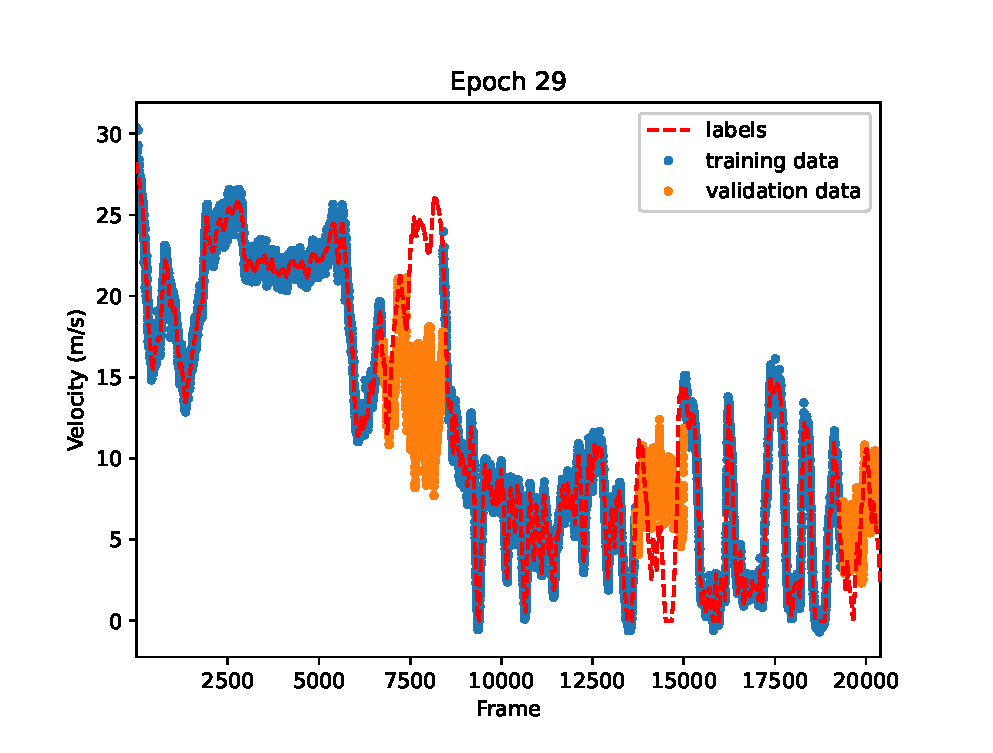
\includegraphics[width=\textwidth]{imgs/siamese_fof_performance.eps}
		\end{column}
	\end{columns}
\end{frame}

\begin{frame}{Siamese Architecture: Performance}
	\textbf{Performance (Siamese network with two frames):}
	\begin{columns}[c]
		\begin{column}{0.5\textwidth}
			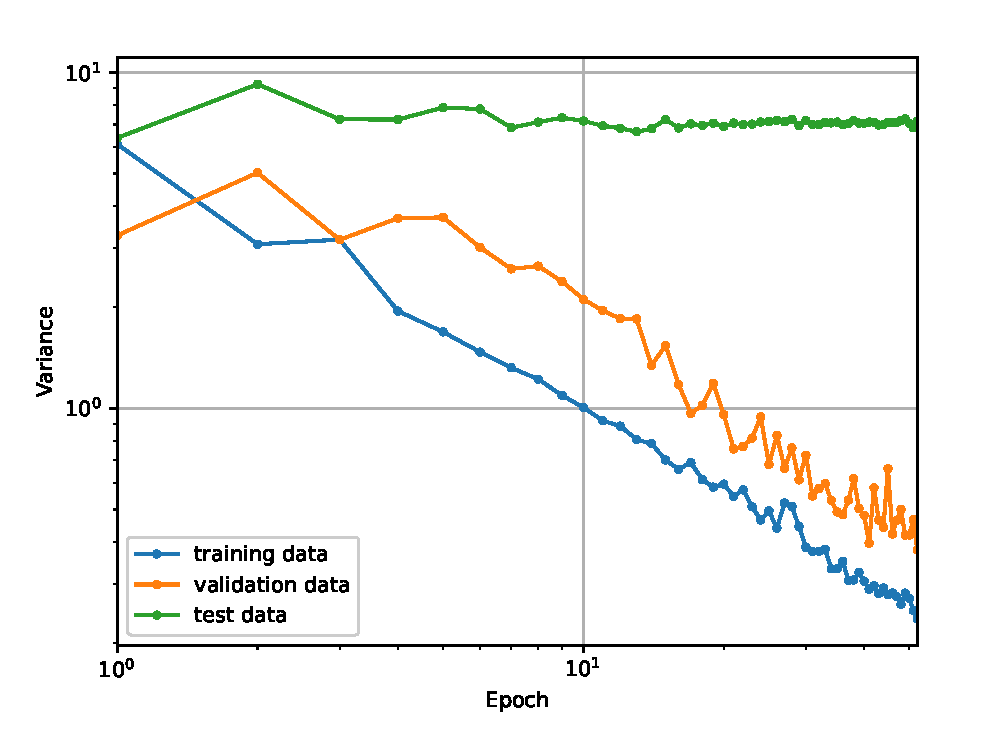
\includegraphics[width=\textwidth]{imgs/siamese_training.eps}
		\end{column}
		\begin{column}{0.5\textwidth}
			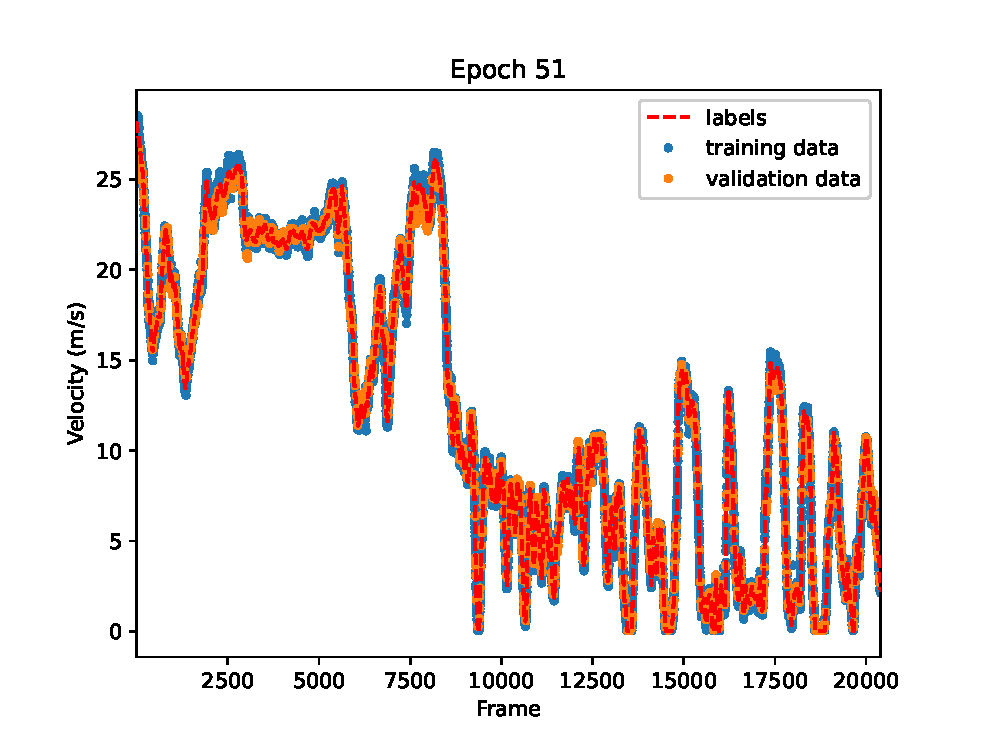
\includegraphics[width=\textwidth]{imgs/siamese_performance.eps}
		\end{column}
	\end{columns}
\end{frame}

\subsection{Problems and possible solutions}
\begin{frame}{Problems}
We identified two problems
\begin{enumerate}
	\item Overfitting, when validation data is not randomly distributed in the data but a of continuous blocks
	\item Predictions are very susceptible for brightnesses/illumination changes in the frames, because of unstable calculations of the optical flow
\end{enumerate}
\begin{columns}[c]
	\begin{column}{0.5\textwidth}
		\begin{center}
		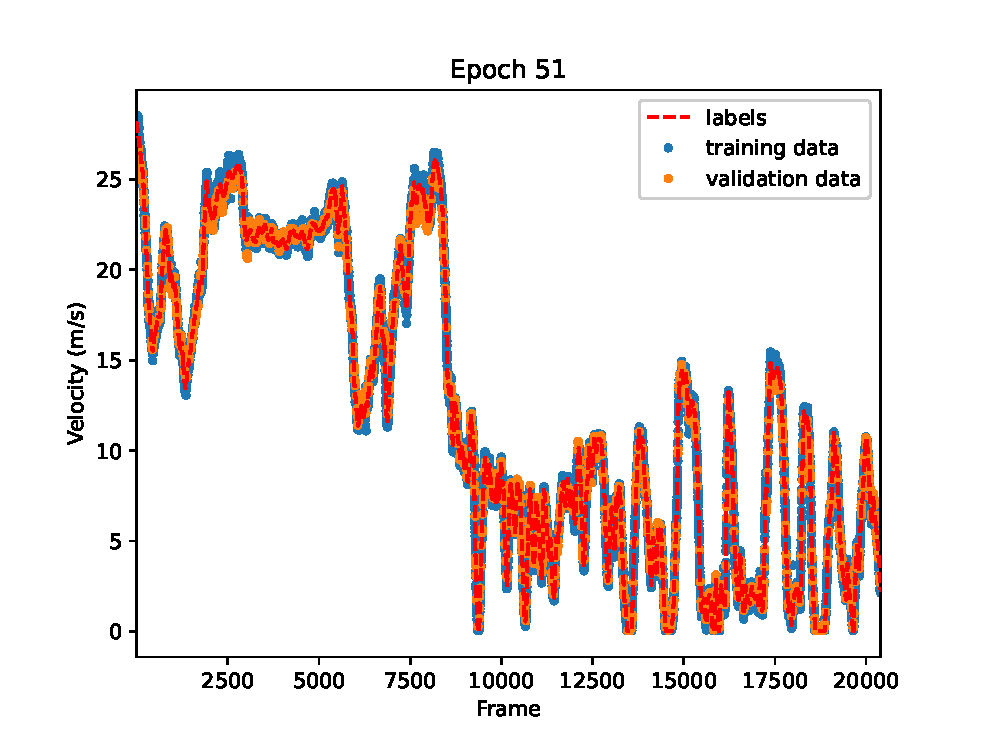
\includegraphics[width=\textwidth]{imgs/siamese_performance.eps}
		random shuffled validation data
		\end{center}
	\end{column}
	\begin{column}{0.5\textwidth}
		\begin{center}
		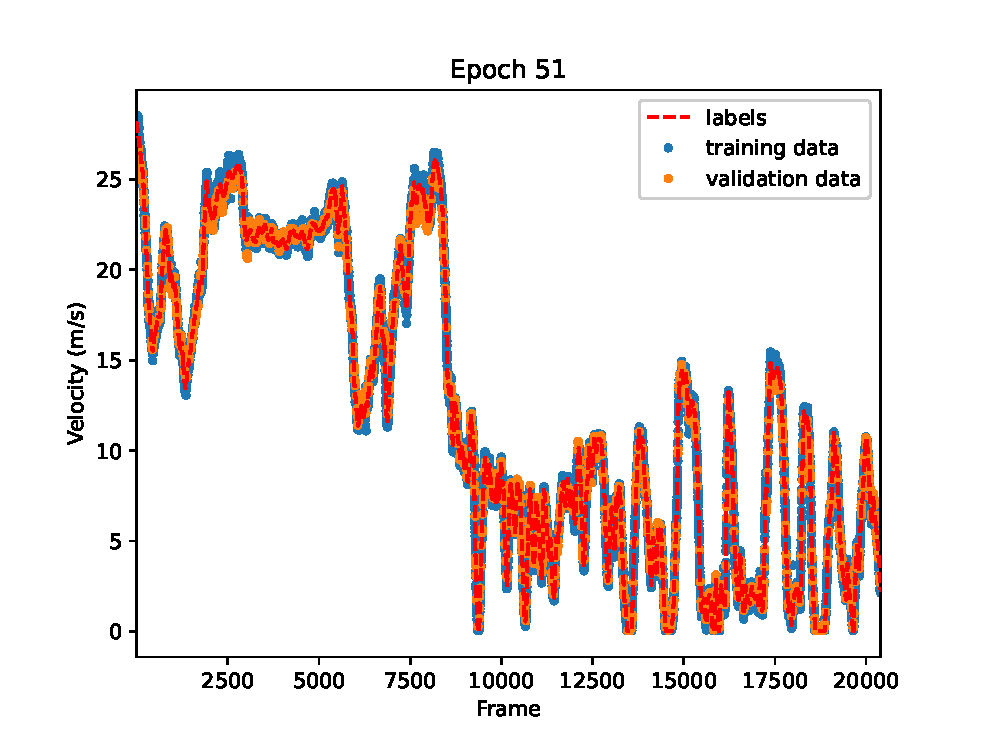
\includegraphics[width=\textwidth]{imgs/siamese_performance.eps}
		block validation data
		\end{center}
	\end{column}
\end{columns}
\end{frame}

\begin{frame}{Problems and possible solutions}
\textbf{Problems}
\begin{itemize}
	\item Predictions are limited to data very similar to the training data
	\item Predictions do not generalize well
\end{itemize}
\textbf{Most likely explanations:}
\begin{itemize}
	\item Very limited dataset for a complex model
	\item Network is not prepared for unseen situations
	\item Changes in brightness and illumination
\end{itemize}
\textbf{Solution:}
\begin{itemize}
	\item Acquire more data for various driving situations and/or use a less complex model
%	\item use a technique to normalize different brightnesses
	\item Add noise to the data, more robustness in the optical flow calculation
%	\item Use a less complex model
\end{itemize}
\end{frame}

%\begin{frame}{Possible solutions}
%\textbf{Process of detecting speed from a video}
%\begin{itemize}
%	\item extracting features from each frame
%	\item check how the features have moved between two frames
%	\item evaluate if the movement comes from own speed or other sources
%\end{itemize}
%
%$\Rightarrow$ for good generalization a complex model is necessary
%
%\textbf{Solutions:}
%\begin{itemize}
%	\item acquire more data for various driving situations
%	\item use a technique to normalize different brightnesses
%	\item add randomly noise to the data to negate wrong features
%	\item use a much less complex model
%\end{itemize}
%\end{frame}

\begin{comment}	
\begin{enumerate}
\item \textbf{Simplify model}: pooling layers (maximum and average pooling) to get more compression\\
\textbf{Siamese approach}: put flow field and raw frame into the model or put two consecutive frames into the model
\item \textbf{Add additional noise}: add noise before computing the optical flow filed, to get more invariance regarding illumination changes
\item \textbf{Different splitting}: get better ratio between different scenarios, by using a splitting based on the different road traffic situations in the video
\end{enumerate}
\end{frame}


\begin{frame}{New splitting: situational splitting}
\begin{figure}
\centering
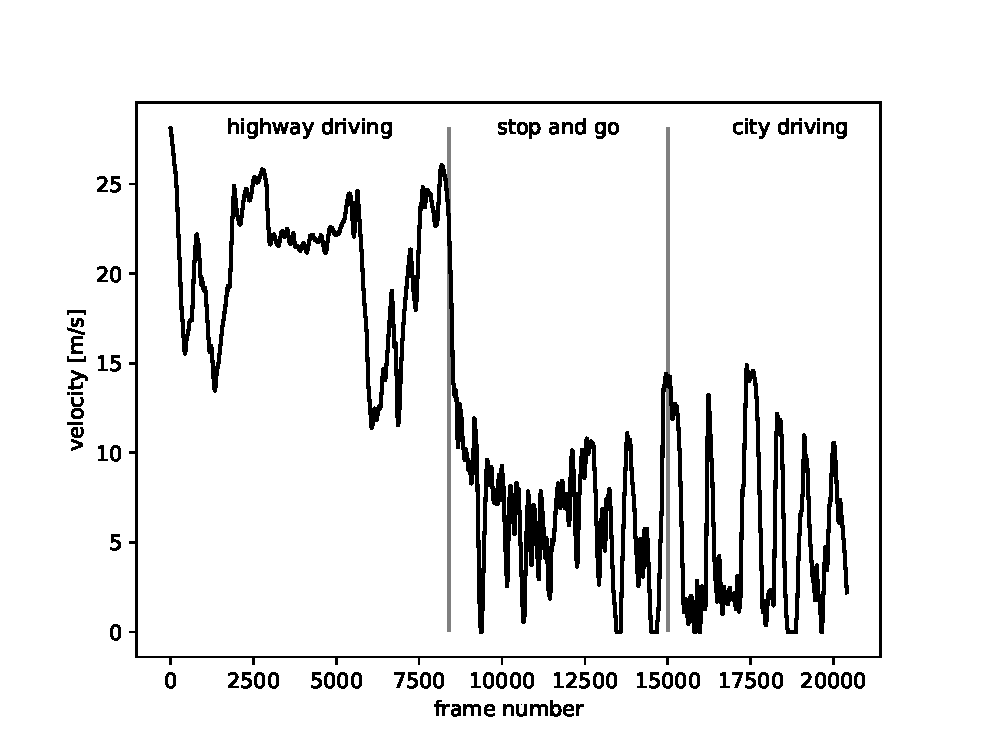
\includegraphics[scale=0.5]{./imgs/plot_speed_time_new_splitting.eps}
\caption{Velocity distribution in the training video, including labels for different scenarios.}
\end{figure}
\end{frame}
\end{comment}

